\documentclass{standalone}
\usepackage{tikz}
% \usepackage{amsmath}
% \DeclareMathOperator{\Real}{Re}
% \DeclareMathOperator{\Imag}{Im}
\begin{document}
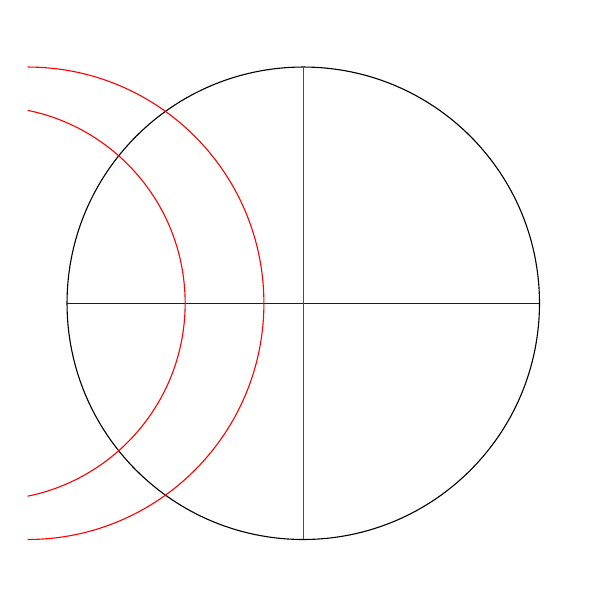
\begin{tikzpicture}
\clip (-3.5,-3.5) rectangle (3.5,3.5);

\draw (0,0) circle [radius=3];

\draw[color=blue] (-3,0) -- (3,0);
% \draw[color=blue] (-3,0) to[out=30, in=150] (3,0);
% \draw[color=blue] (-3,0) to[out=60, in=120] (3,0);
% \draw[color=blue] (-3,0) to[out=90, in=90] (3,0);
% \draw[color=blue] (-3,0) .. controls (0,1) .. (3,0);
% \draw[color=blue] (-3,0) .. controls (0,2) .. (3,0);
% \draw[color=blue] (-3,0) .. controls (0,3) .. (3,0);

\draw[color=red] (0,-3) -- (0,3);
\draw[color=red] (-3.5,0) circle [radius=3];
\draw[color=red] (-4,0) circle [radius=2.5];
%
% \foreach \x in {-1,...,1}
% \foreach \y in {-1,...,1}
%   \fill[color=blue] (2*\x,2*\y) circle (0.05);
%
% \foreach \x in {-2,...,1}
% \foreach \y in {-2,...,1}
%   \fill[color=blue] (2*\x+1,2*\y+1) circle (0.05);
%
% \draw[->, thick] (0,0) -- node[right]{$\kappa_1$} (1,-1);
% \draw[->, thick] (0,0) -- node[left]{$\kappa_2$} (-1,-1);
\end{tikzpicture}
\end{document}
